
In the proposed architecture, the SmartBox plays the role of acquiring the data that is transmitted wirelessly by the Biostickers.
Each SmartBox is associated with a single patient, and captures the data of each Biosticker associated with that patient. 

\section{Deciding on a Hardware Platform}

In the context of the dissertation, two different \acl{SBC}s (\acs{SBC}) were considered for the development of the SmartBox: a Raspberry Pi 4 Model B and an UDOO BOLT v3. In the following sections we will discuss and compare the characteristics of each platform. 

\subsubsection{Raspberry Pi 4 Model B}

Raspberry Pi denotes a series of \acs{SBC}s which are developed by the Raspberry Pi Foundation, a UK-based charity that aims to educate the general public about the power of computing and digital making, in association with Broadcom. It is one of the most popular hardware platforms used by developers due to its accessible price and community support.
At the time of the writing of this dissertation, the Raspberry Pi 4 Model B is the latest revision of the Raspberry Pi series, powered by Broadcom BCM2711 System on a Chip (SoC).

\begin{figure}[H]
    \centering
    \includegraphics[width=0.5\linewidth]{images/raspberrypi-image.jpg}
    \caption{Raspberry Pi 4 Model B.}
    \label{fig:raspberrypi-image}
\end{figure}

\subsubsection{UDOO BOLT V3}

As mentioned by the manufacturer\footnote{Product Website: https://www.udoo.org/discover-the-udoo-bolt/}, the ``UDOO BOLT is a quantum leap compared to current maker boards''. It represents a series of high performance \acs{SBC}, equipped with the latest generation of AMD Ryzen Embedded SoC. Additionally, it contains an Arduino Compatible microcontroller (connected via UART), making it the UDOO BOLT extremely versatile with its.
The UDOO Bolt is incredibly well supported by UDOO. And since it runs desktop Linux distros and Windows 10, third-party support is top-notch. Unfortunately, it doesn't have nearly the same community support of Raspberry Pi.

The UDOO BOLT V3 is the entry-level product of the series, but it is still capable of outperforming full-fledged computers such as the Apple MacBook 13", which just goes to show how powerful these \acs{SBC}s can be.

\begin{figure}[H]
    \centering
    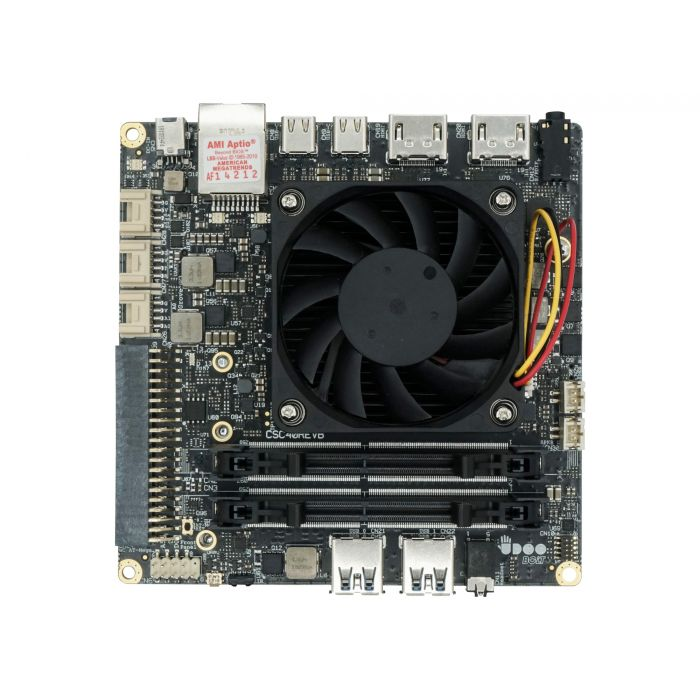
\includegraphics[width=0.5\linewidth]{images/udoobolt-image.jpg}
    \caption{Udoo Bolt V3.}
    \label{fig:udoobolt-image}
\end{figure}

\subsection{Comparing the Hardware Platforms}

From the table \ref{tab:comparsion-hardwareplatform}, we can infer that the Raspberry Pi is a much more affordable alternative.

\renewcommand{\arraystretch}{2}
\begin{table}[H]
    \centering
    \begin{tabular}{r|l|l}
        %\textbf{Features} 
        & \textbf{Raspberry Pi 4B}& \textbf{Udoo Bolt V3}  \\ \hline
        \textbf{SoC} &  \makecell{Broadcom BCM2711 (ARM v8 \\ 64-bit) 4-core @ 1.5GHz} & \makecell{AMD Ryzen™ Embedded V1202B (x86-64) \\ 2-core @ 2.3GHz (up to 3.2GHz turbo)}\\
        \textbf{RAM} & 2, 4 or 8 GB LPDDR4 & Up to 32GB DDR4 (Not included) \\ 
        \textbf{Storage} & \makecell{No internal storage, \\ SDXC Card Support} & \makecell{32GB internal eMMC + \\1x SATA III and 2x M.2 connectors}\\
        \textbf{Networking} & \makecell{2.4/5.0 GHz WiFi, Gigabit \\ Ethernet, Bluetooth 5.0, BLE} & \makecell{Gigabit Ethernet + M.2 Key E slot \\ for optional WiFi+BT module}\\ 
        \textbf{I/O Ports} & 2 × USB 3.0, 2 × USB 2.0 & \makecell{2x USB 3.0 Type-A, 2x USB Type-C (w/ \\ Display Port + Power Delivery), 2x HDMI} \\
        \makecell[r]{\textbf{Other} \\\textbf{Features}} & Power over Ethernet (PoE)–enabled & \makecell{Includes ATmega32U4 microcontroller\\ (Arduino Leonardo compatible), \\ RTC Battery} \\   
        \textbf{Dimensions} & 0.85 x 0.56 x 0.17 cm & 12 x 12 x 7 cm \\
        \textbf{Price} & \makecell{61,73 € (including 32GB SDXC Card\\ and case)} & \makecell{534.48 € (including external power supply\\ and 16GB RAM module)} \\
    \end{tabular}
    \caption{Comparison of the specifications of the Raspberry Pi 4B and Udoo Bolt V3.}
    \label{tab:comparsion-hardwareplatform}
\end{table}
\renewcommand{\arraystretch}{1}


In order to understand the differences in performance between these two platforms, a test suite was developed and conducted. The tools developed for each test can be found in \url{https://github.com/WoW-Institute-of-Systems-and-Robotics/smartbox_benchmark_tests}. 

In the next sections, we detail how each test works and discuss how each \acs{SBC} performed. 

\subsubsection{Test 1: \textit{7-Zip} CPU Benchmark}
\dots

\subsubsection{Test 2: Python Benchmark}
In this test, the hardware platforms ran simple Python scripts 

\begin{figure}[H]
    \centering
    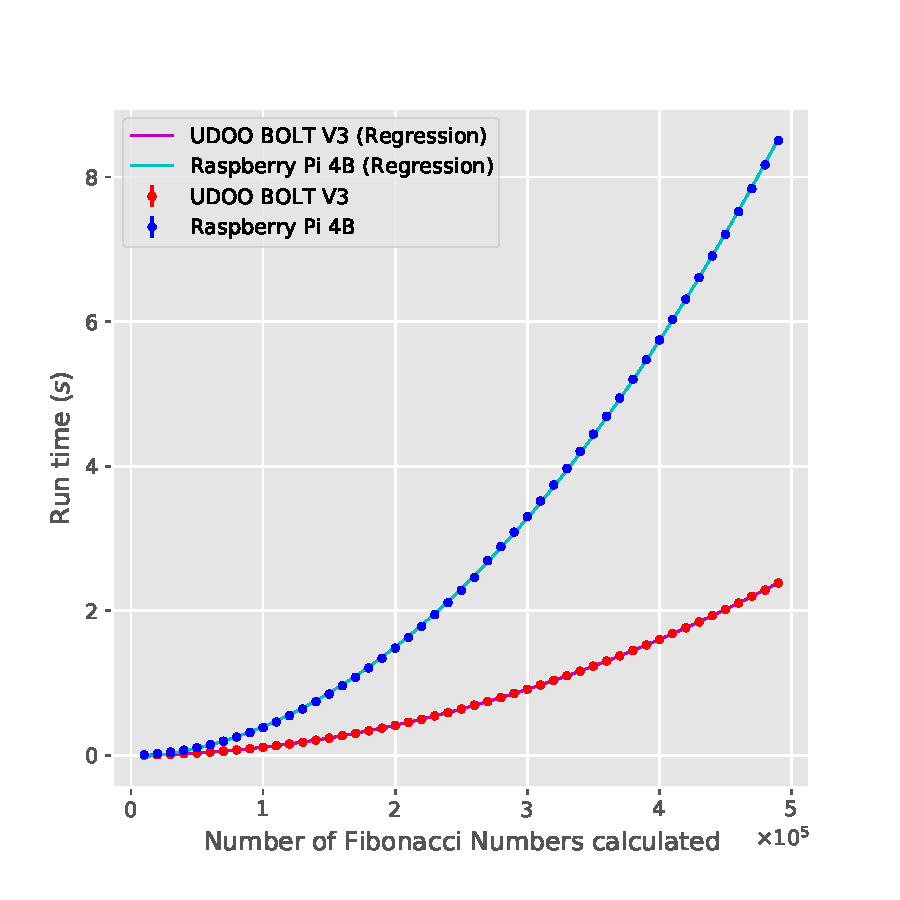
\includegraphics[width=0.6 \linewidth]{images/fibonacci-test.pdf}
    \caption{Results of our custom Python benchmark. }
    \label{fig:fibonacci-tests}
\end{figure}

\subsubsection{Test 3: Phoronix Test Suite}
The Phoronix Test Suite\footnote{Phoronix Test Suite - Linux Testing \& Benchmarking Platform, Automated Testing, Open-Source Benchmarking: \textit{https://www.phoronix-test-suite.com/}} is an open-source benchmarking platform used for comparing the performance of different systems. The framework provides compilations of tests for a variety of tools and is also fully customizable and expandable, allowing users to develop and automate their own tests in a clean, reproducible and easy-to-use fashion.  

For the purposes of evaluating which single board computer should be used, we chose the Python and CPU tests provided by Phoronix\footnote{OpenBenchmarking.org - Cross-Platform, Open-Source Automated Benchmarking Platform: \textit{https://openbenchmarking.org/}}. These tests provide a quantitative score describing the \acs{SBC} performance during the test, 


\subsubsection{Test 4: \acs{MQTT} Benchmark}
As the Smartbox will communicate with the Smart Gateway through \acs{MQTT}, we decided to evaluate how each system handles the load associated with an MQTT client. For this test, each \acs{SBC} ran a simple \acs{MQTT} client which was subscribing to a single topic and publishing to another topic.

\begin{figure}[H]
    \centering
    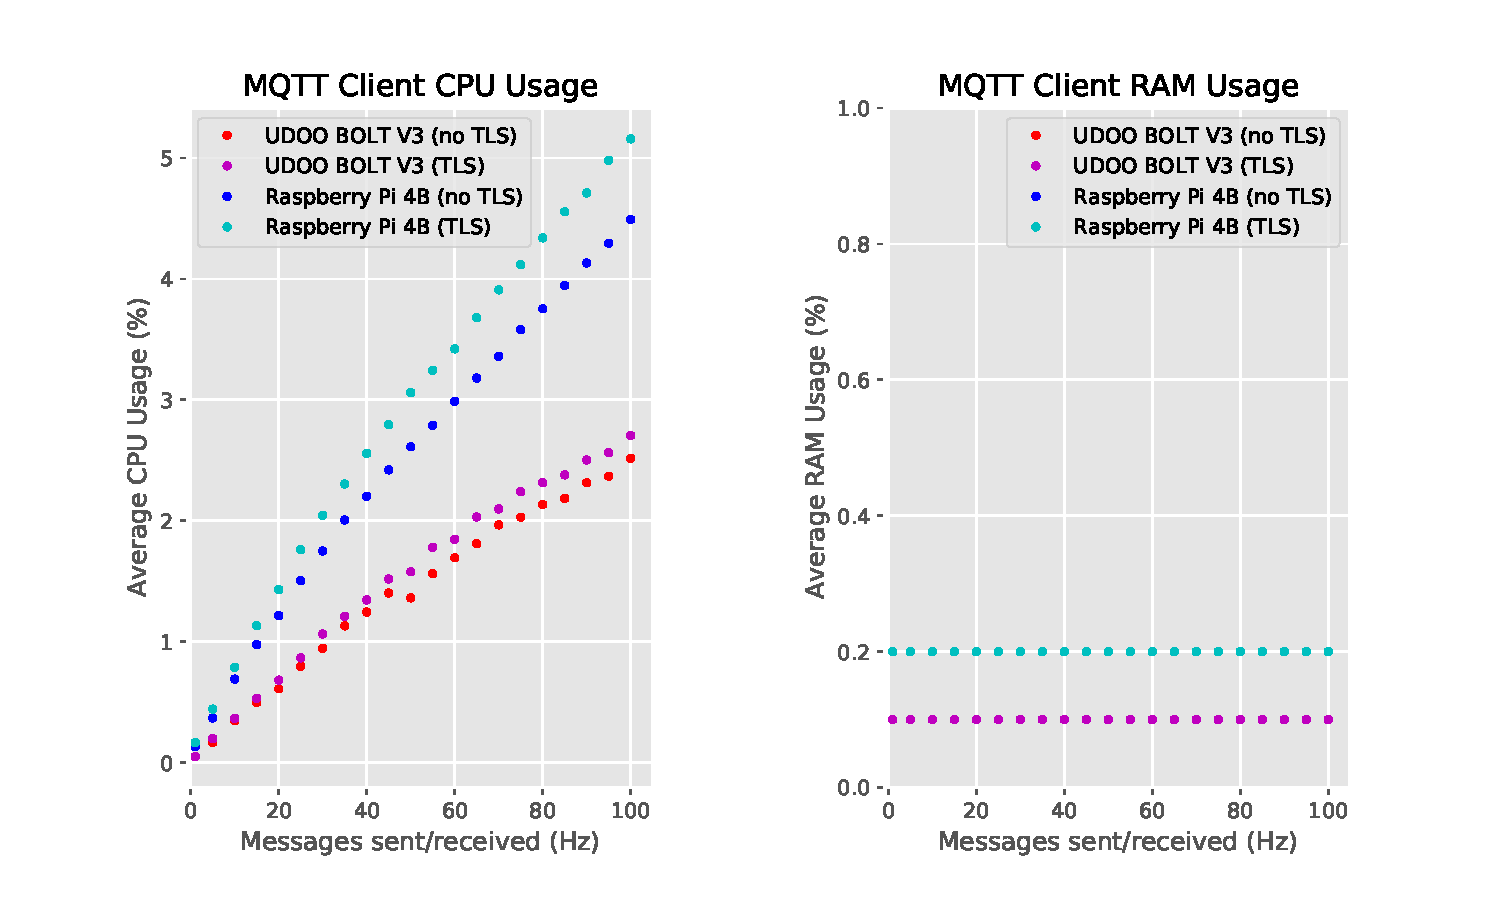
\includegraphics[width=\linewidth]{images/mqtt_test_results.pdf}
    \caption[Results of the MQTT benchmark.]{Results of the MQTT benchmark. As the transmission frequency increases, we observe that the Raspberry Pi consumes more resources than the UDOO BOLT V3, nonetheless, these are very negligible performance differences, with an impact of < 0.5\% resource usage.}
    \label{fig:mqtt-tests}
\end{figure}

As expected, the \acs{MQTT} client is a very lightweight process, and therefore should be capable of running on both platforms with trivial impact.

\subsubsection{Conclusion}

Based on the results of our tests we conclude that Udoo Bolt V3 outperforms the Raspberry Pi 4 Model B by a factor of 3 in CPU benchmarks, and shows a negligible performance difference in memory usage. However, the Raspberry Pi provides a much better value, since its cost is much lower than an Udoo Bolt V3 (over 1/5 the cost, accounting for the RAM modules). Not only that, but we find that these performance gains do not meaningfully impact the SmartBox functionality, for example, the MQTT communication, which further 
reinforces our decision.

\section{Communication with the Biostickers}

\subsection{Overview of \acf{BLE}}

\begin{figure}[H]
    \centering
    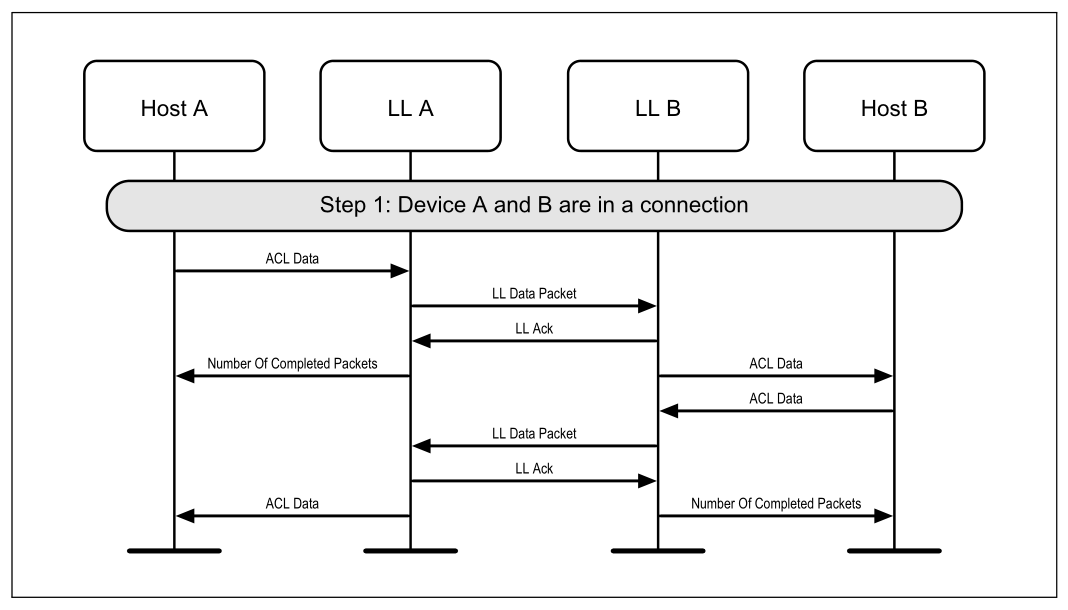
\includegraphics[width=\linewidth]{images/ble-sending-data.PNG}
    \caption[Message sequence chart between two \acs{BLE} devices sending data and replying to the request.]{Message sequence chart between two \acs{BLE} devices sending data and replying to the request. Source: \cite{Specification1999}}
    \label{fig:differences-between-cloud-services}
\end{figure}


\begin{enumerate}
    \item Slave Latency:
    \item Connection Interval:
    \item Supervisor Timeout
    \item \acs{MTU} for the \acs{ATT} protocol: 
\end{enumerate}

\subsubsection{Test 1: Roundtrip Time Measurement}

\subsubsection{Test 2: Bandwidth Measurement}


\section{Summary}
In this chapter, we \dots